\documentclass{beamer}

\usepackage[T2A]{fontenc}
\usepackage[utf8x]{inputenc}
\usepackage[english,bulgarian]{babel}
\usepackage{multirow}

\mode<presentation> {
	\usetheme{Berlin}
}

%\usebackgroundtemplate {
%	\includegraphics[width=370px, height=270px, trim=0 0 0 -80px]{background}
%}

\graphicspath{{../images/}}

\title{Оператори за контрол на изпълнението и потребителски функции}
\subtitle{Статистическа обработка на данни с R}

\author{Пламен Петров и Тодор Балабанов}

\date{22.V.2020}

\institute[ЦО и ИИКТ към БАН] {
	Център за обучение \\
	Институт по информационни и комуникационни технологии \\ 
	Българската академия на науките \\
	\medskip
	\textit{p.petrov@iit.bas.bg todorb@iinf.bas.bg}
}

\addtobeamertemplate{navigation symbols}{}{
	\usebeamerfont{footline}
	\usebeamercolor[fg]{footline}
	\hspace{1em}
	\insertframenumber/\inserttotalframenumber
}

\begin{document}

\begin{frame}
	\titlepage
\end{frame}

\section*{Теми}
\begin{frame}[shrink]
	\frametitle{Съдържание}
	\tableofcontents
\end{frame}

\section{Организация на експериментите}

\begin{frame}
\center \huge{Организация на експериментите}
\end{frame}

\subsection{Скриптови езици}

\begin{frame}
\frametitle{Последователност от инструкции}
\begin{block}{Примерен R скрипт}
rm(list = ls());

sayHello <- sample(c(TRUE,FALSE), 1, TRUE);

if(sayHello == TRUE) \{

	print( $"$Hello!$"$ );
	
\}

print( $"$Bye!$"$ );
\end{block}

\begin{block}{Адрес на скрипта}
https://raw.githubusercontent.com/TodorBalabanov/Statistical-Data-Processing-with-R/master/code/example0001.r
\end{block}
\end{frame}

\begin{frame}
\frametitle{Текстов редактор към продукта R}
\begin{figure}[]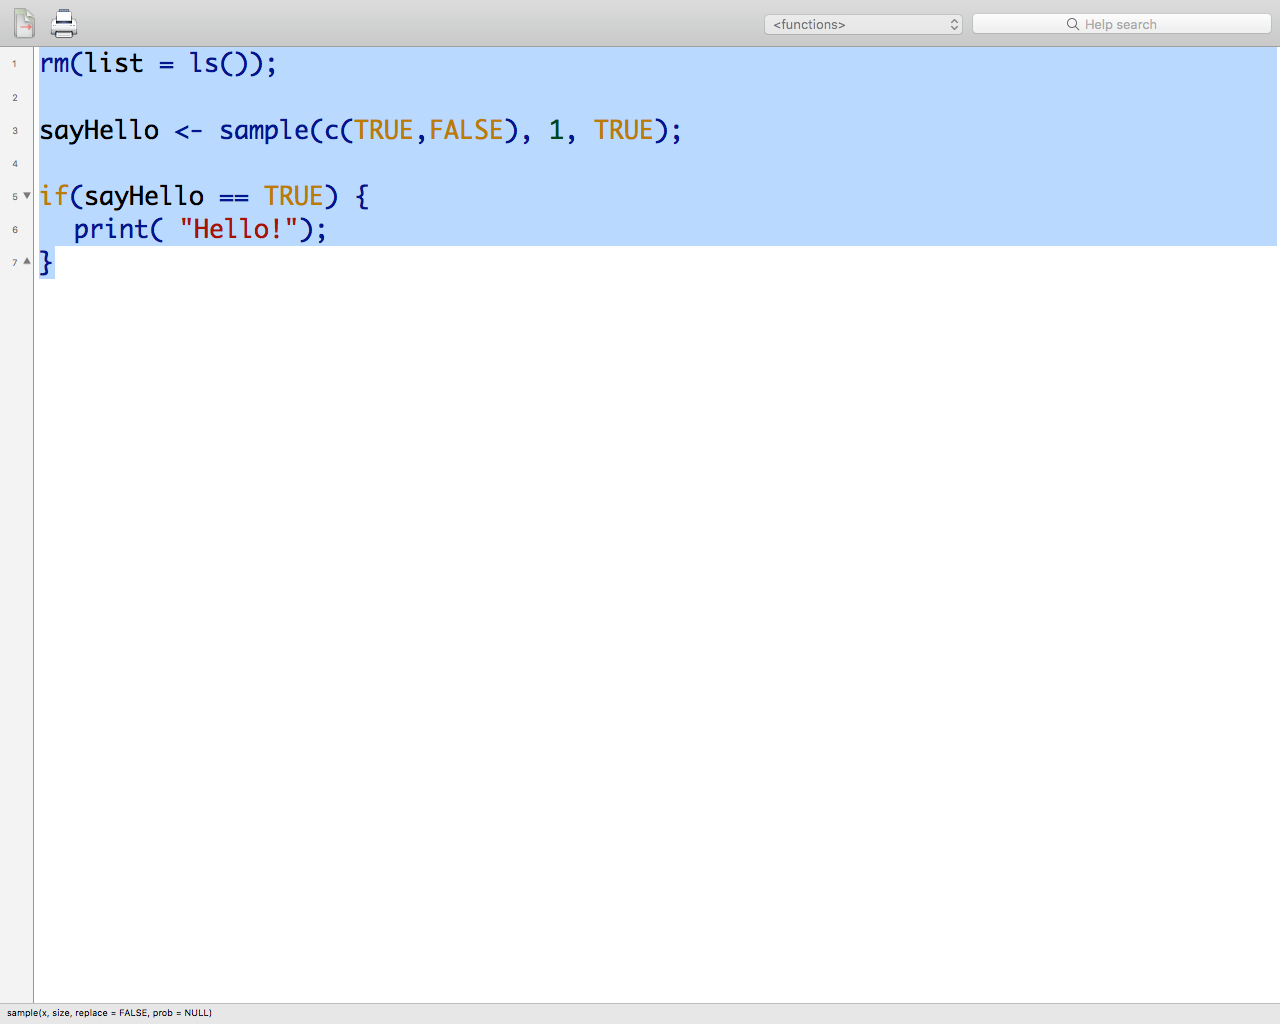
\includegraphics[width=\textwidth,height=0.75\textheight]{pic0025}\end{figure}
\end{frame}

\begin{frame}
\frametitle{Стартиране на R скрипт}
\begin{figure}[]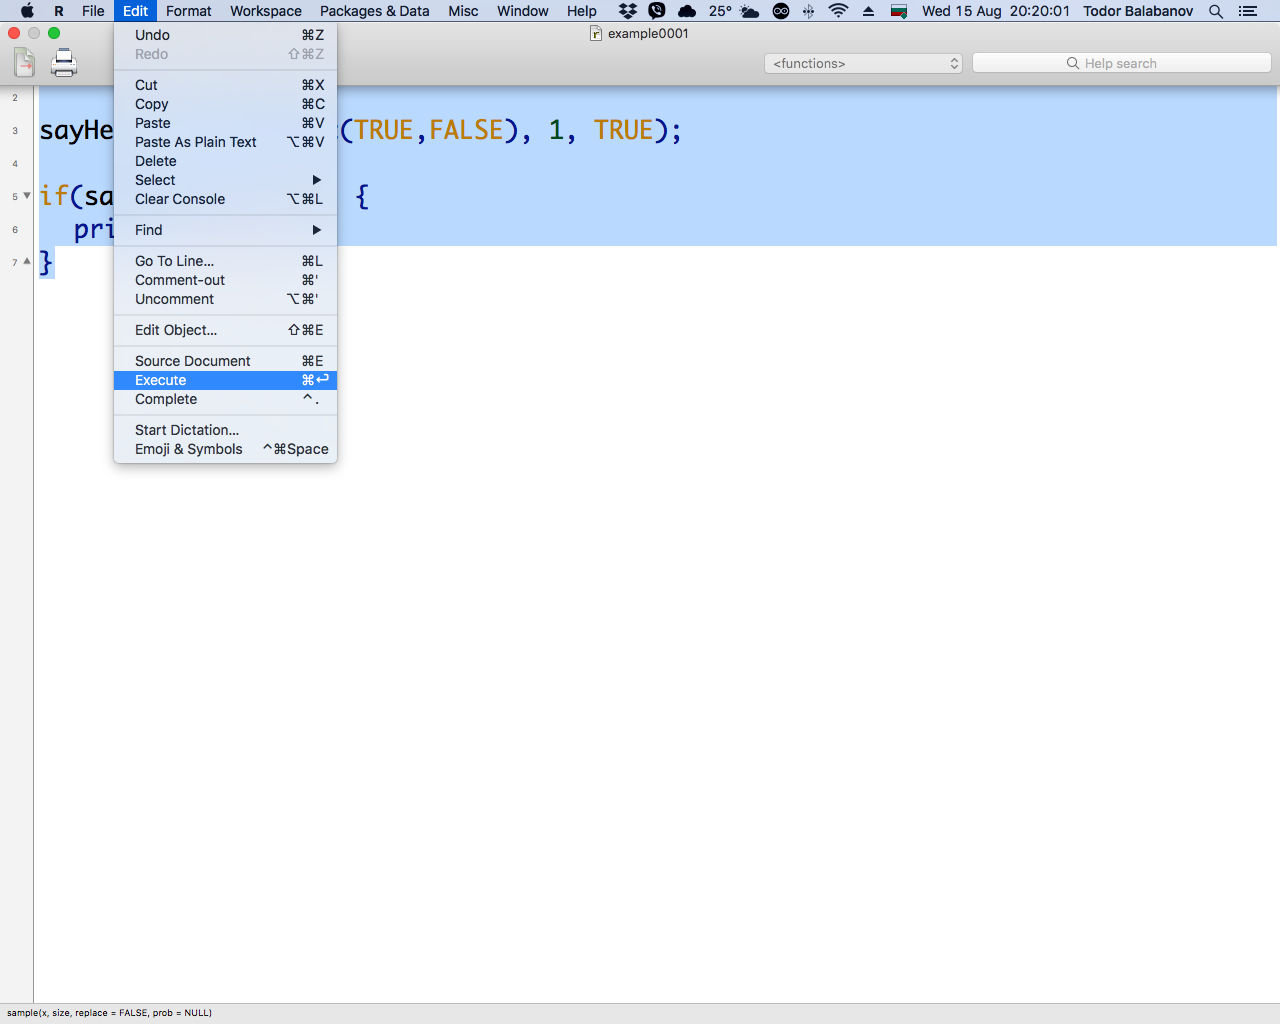
\includegraphics[width=\textwidth,height=0.75\textheight]{pic0026}\end{figure}
\end{frame}

\begin{frame}
\frametitle{Резултат от изпълнението на R скрипт}
\begin{figure}[]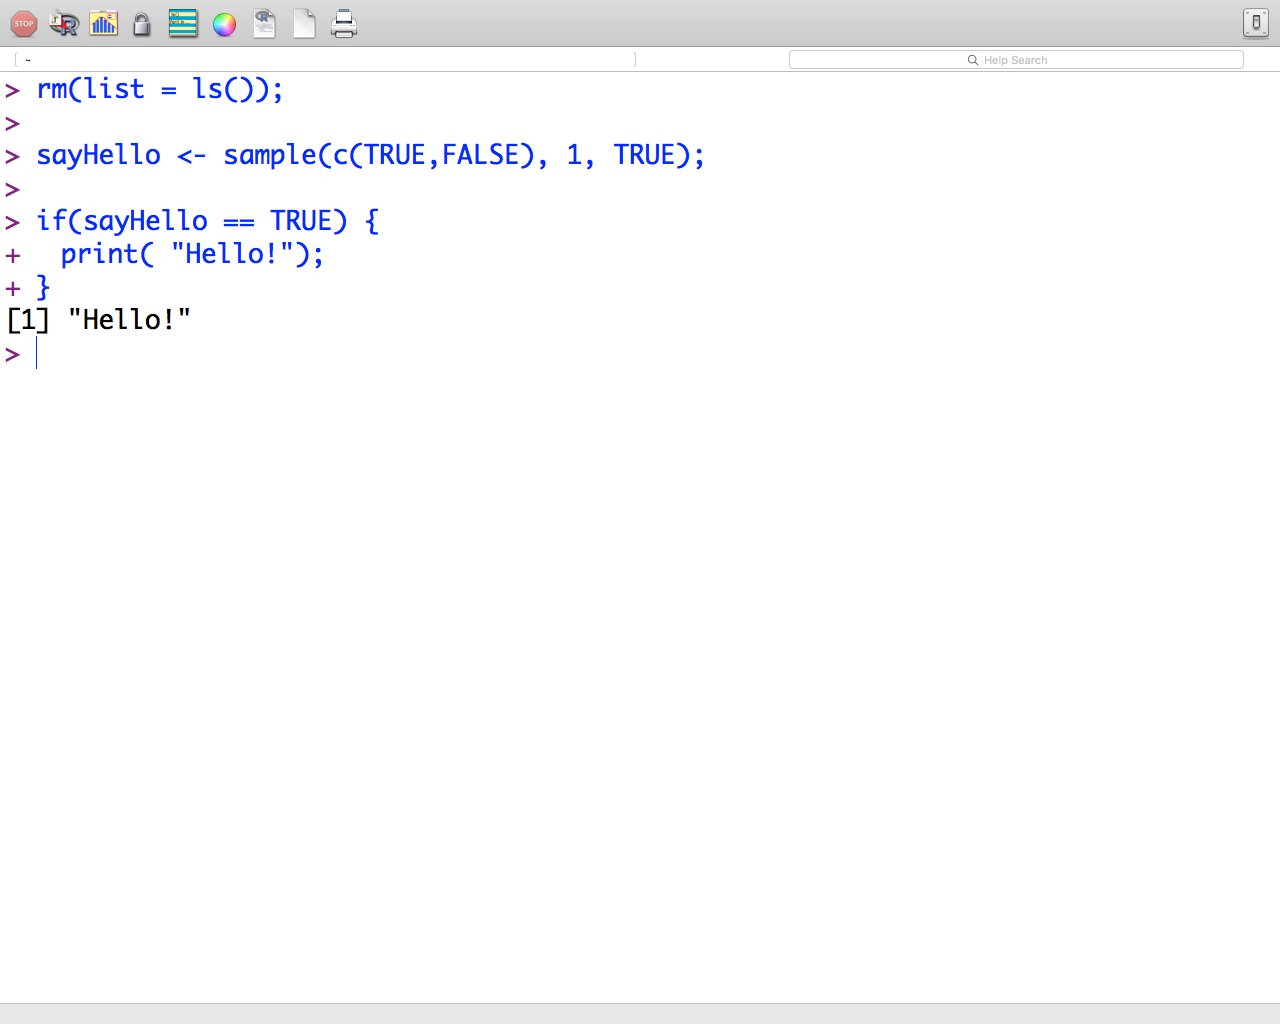
\includegraphics[width=\textwidth,height=0.75\textheight]{pic0027}\end{figure}
\end{frame}

\begin{frame}
\frametitle{Резултат от изпълнението на R скрипт в конзолата на операционната система}
\begin{figure}[]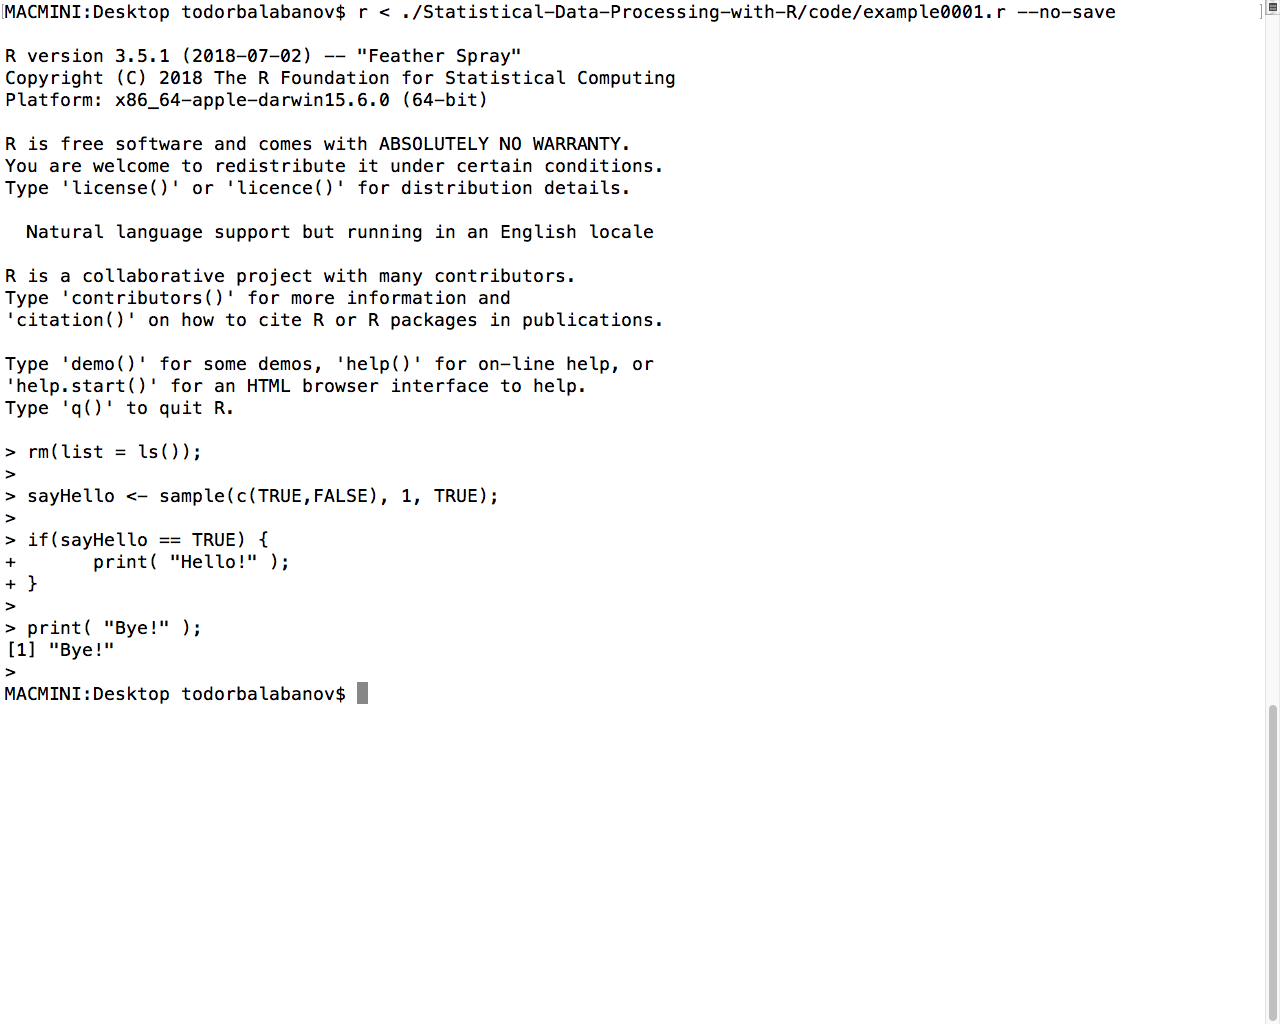
\includegraphics[width=\textwidth,height=0.75\textheight]{pic0028}\end{figure}
\end{frame}

\section{Оператори за преход}

\begin{frame}
\center \huge{Оператори за преход}
\end{frame}

\subsection{Оператор за условен преход}

\begin{frame}
\frametitle{Избор на инструкции}
\begin{block}{Оператор за условен преход if}
sayHello <- sample(c(TRUE,FALSE), 1, TRUE);

if(sayHello == TRUE) \{

	print( $"$Hello!$"$ );
	
\}

print( $"$Bye!$"$ );
\end{block}
\end{frame}

\subsection{Алтернатива при условен преход}

\begin{frame}
\frametitle{Алтернативи при избор}
\begin{block}{Оператор за условен преход if-else}
sayHello <- sample(c(TRUE,FALSE), 1, TRUE);

if(sayHello == TRUE) \{

	print( $"$Hello!$"$ );

\} else \{

	print( $"$Hi!$"$ );

\}

print( $"$Bye!$"$ );
\end{block}
\end{frame}

\subsection{Каскада от условни преходи}

\begin{frame}
\frametitle{Множество от алтернативи}
\begin{block}{Каскада от if-else}
sayHello <- sample(c(0,1,2), 1, TRUE);

if(sayHello == 0) \{

	print( $"$Hello!$"$ );

\} else if(sayHello == 1) \{

	print( $"$Hi!$"$ );

\} else if(sayHello == 2) \{

	print( $"$Yoo!$"$ );

\} else \{

	print( $"$Error!$"$ );

\}

print( $"$Bye!$"$ );
\end{block}
\end{frame}

\begin{frame}
\frametitle{Множество от алтернативи}
\begin{block}{Функцията ifelse}
ifelse(sample(c(FALSE,TRUE), 1, TRUE), $"$Yes$"$, $"$No$"$)

ifelse(c(1,1,0,1,0,1)==1, $"$Yes$"$, $"$No$"$)
\end{block}
\end{frame}

\subsection{Оператор за многовариантен избор}

\begin{frame}
\frametitle{Множесво възможности}
\begin{block}{Конструкция за многовариантен избор switch}
switch(sample(c($"$a$"$,$"$b$"$,$"$c$"$,$"$d$"$,$"$e$"$),1,TRUE), $"$a$"$=$"$one$"$, $"$b$"$=$"$two$"$, $"$c$"$=$"$three$"$, $"$d$"$=$"$four$"$, $"$other$"$)
\end{block}
\end{frame}

\section{Оператори за цикъл}

\begin{frame}
\center \huge{Оператори за цикъл}
\end{frame}

\subsection{Цикъл за обхождане}

\begin{frame}
\frametitle{Оператор за цикъл for}
\begin{block}{Обхождане по числен диапазон}
for(number in 1:10) \{ 

	print(number); 
	
\}
\end{block}

\begin{block}{Обхождане по вктор от символни низове}
for(f in c($"$orange$"$, $"$lemon$"$, $"$kiwi$"$, $"$cherry$"$)) \{ 

	print(f); 

\}
\end{block}
\end{frame}

\subsection{Цикъл с условие за край}

\begin{frame}
\frametitle{Цикъл с предусловие}
\begin{block}{Цикъл с условие за край}
counter <- 1;

while(counter <= 5) \{ 

	print( counter ); 
	
	counter <- counter + 1;

\}
\end{block}
\end{frame}

\subsection{Прекъсване на циклите}

\begin{frame}
\frametitle{Частично прекъсване}
\begin{block}{Прекъсване на итерация}
for(number in 1:10) \{ 

	if(number == 7) \{
	
		next;
		
	\}

	print(number);
	
\}
\end{block}
\end{frame}

\begin{frame}
\frametitle{Пълно прекъсване}
\begin{block}{Прекъсване на цикъла}
for(number in 1:10) \{ 

	if(number == 3) \{
	
		break;
		
	\}

	print(number);

\}
\end{block}
\end{frame}

\section{Потребителски функции}

\begin{frame}
\center \huge{Потребителски функции}
\end{frame}

\subsection{Аргументи на функция}

\begin{frame}
\frametitle{Организация на група от команди}
\begin{block}{Примерна потребителска функция}
say.hello <- function() \{

	print( $"$Hello, World!$"$ );

\}

say.hello();
\end{block}
\end{frame}

\begin{frame}
\frametitle{Параметризиране на групата инструкции}
\begin{block}{Извикване на функция с аргумент}
hello.person <- function( name ) \{

	print( sprintf( $"$Hello, \%s!$"$, name) );

\}

hello.person( $"$Dessislava$"$ );
\end{block}
\end{frame}

\begin{frame}
\frametitle{Параметризиране на групата инструкции}
\begin{block}{Извикване на функция с повече аргументи}
hello.person <- function(first, last) \{

	print( sprintf($"$Hello, \%s \%s!$"$, first,last) );

\}

hello.person( $"$Dessislava$"$, $"$Gruncharova$"$ );

hello.person( last = $"$Mladevnova$"$, first = $"$Vyara$"$);
\end{block}
\end{frame}

\subsection{Аргументи с подразбираща се стойност}

\begin{frame}
\frametitle{Не задължителни аргументи}
\begin{block}{Извикване на функция с подразбиращи се аргументи}
hello.person <- function(first, last, title=$"$$"$) \{

	print( sprintf( $"$Hello, \%s \%s \%s!$"$, title, first, last ) );

\}

hello.person( $"$Zornitsa$"$, $"$Radeva$"$, $"$Miss$"$ );

hello.person( $"$Todor$"$, $"$Balabanov$"$ );
\end{block}
\end{frame}

\subsection{Променлив брой аргументи}

\begin{frame}
\frametitle{Не задължителни аргументи}
\begin{block}{Функция с променлив брой аргументи}
sum.up <- function(a, b, ...) \{

	print( a+b );

\}

sum.up(1, 2, 3, 4);
\end{block}
\end{frame}

\subsection{Върната стойност}

\begin{frame}
\frametitle{Изходяща информация}
\begin{block}{Връщане на стойност от функция}
sum.up <- function(a, b, ...) \{

	return(a + b);

\}

print( sum.up(1,2,3,4) );
\end{block}
\end{frame}

\subsection{Предаване на функция като аргумент}

\begin{frame}
\frametitle{Полиморфно поведение}
\begin{block}{Избор на функция за извикване по време на изпълнение}
do.stat <- function(values, calculation) \{

	do.call(calculation, args=list(values));

\}

print( do.stat(1:10,mean) );

print( do.stat(1:10,median) );

print( do.stat(1:10,sd) );
\end{block}
\end{frame}

\section{Заключение}

\begin{frame}
\center \huge{Заключение}
\end{frame}

\subsection{Дискусия}

\begin{frame}
\frametitle{Въпроси и отговори}
\center \huge{Благодаря за вниманието!}
\end{frame}

\end{document}
